\subsection{\'Etude de l'approche hi\'erarchis\'ee : HBase}

Les DHT r\'epondent bien au \emph{lookup} (retrouver rapidement la machine qui d\'etient une cl\'e) dans des syst\`emes o\`u les n\oe uds entrent et sortent fr\'equemment. En revanche, certaines charges exigent une coh\'erence plus stricte (lecture apr\`es \`ecriture fiable), une meilleure persistance (donn\'ees conserv\'ees malgr\'e les pannes) et de bonnes performances de scan (lecture de plages de cl\'es) en plus des \`ecritures. L'approche hi\'erarchis\'ee d'Apache HBase cible pr\'ecis\'ement ce compromis.

%\subsubsection{Introduction au mod\`ele hi\'erarchis\'e}

HBase, construit sur HDFS (\emph{Hadoop Distributed File System}, couche de stockage distribu\'e et r\'epliqu\'e), est une base NoSQL distribu\'ee orient\'ee grands volumes, c'est-\`a-dire une base non relationnelle con\c cue pour monter horizontalement sur plusieurs serveurs. Contrairement aux DHT d\'ecentralis\'ees, HBase adopte un mod\`ele \emph{master-worker} : le Master coordonne le cluster et les workers (RegionServers) servent les donn\'ees. Le \emph{range partitioning} d\'ecoupe les donn\'ees en plages de cl\'es tri\'ees ; chaque \emph{row key} (identifiant de ligne) est donc rout\'ee de mani\`ere d\'eterministe, ce qui favorise les scans s\'equentiels et une coh\'erence forte au niveau ligne.

\subsubsection{Fondamentaux architecturaux de HBase}

Avant de d\'etailler les op\'erations \texttt{PUT}/\texttt{GET}, il est utile de situer les r\^oles des composants principaux. HBase s'appuie sur une architecture en couches : un \textbf{plan de contr\^ole} (HMaster et ZooKeeper) pour l'orchestration, un \textbf{plan de donn\'ees} (RegionServers) pour les acc\`es applicatifs, et une couche de persistance (WAL + HFiles sur HDFS) pour la durabilit\'e.

Dans cette organisation, le client n'interagit pas en continu avec le Master pour chaque requ\^ete. Le Master sert surtout \`a localiser les r\'egions et \`a g\'erer le cycle de vie du cluster (allocation, \`equilibrage, reprise sur panne), tandis que les \'echanges de lecture/\'ecriture se font ensuite directement avec le RegionServer responsable de la plage de cl\'es vis\'ee.

Avant de passer \`a l'analyse d\'etaill\'ee des performances, il est utile d'isoler le cycle d'une requ\^ete d'\'ecriture puis de lecture pour comprendre o\`u se situent le co\^ut de localisation, le chemin de persistance et le point de service de la donn\'ee.

\begin{figure}[H]
\centering
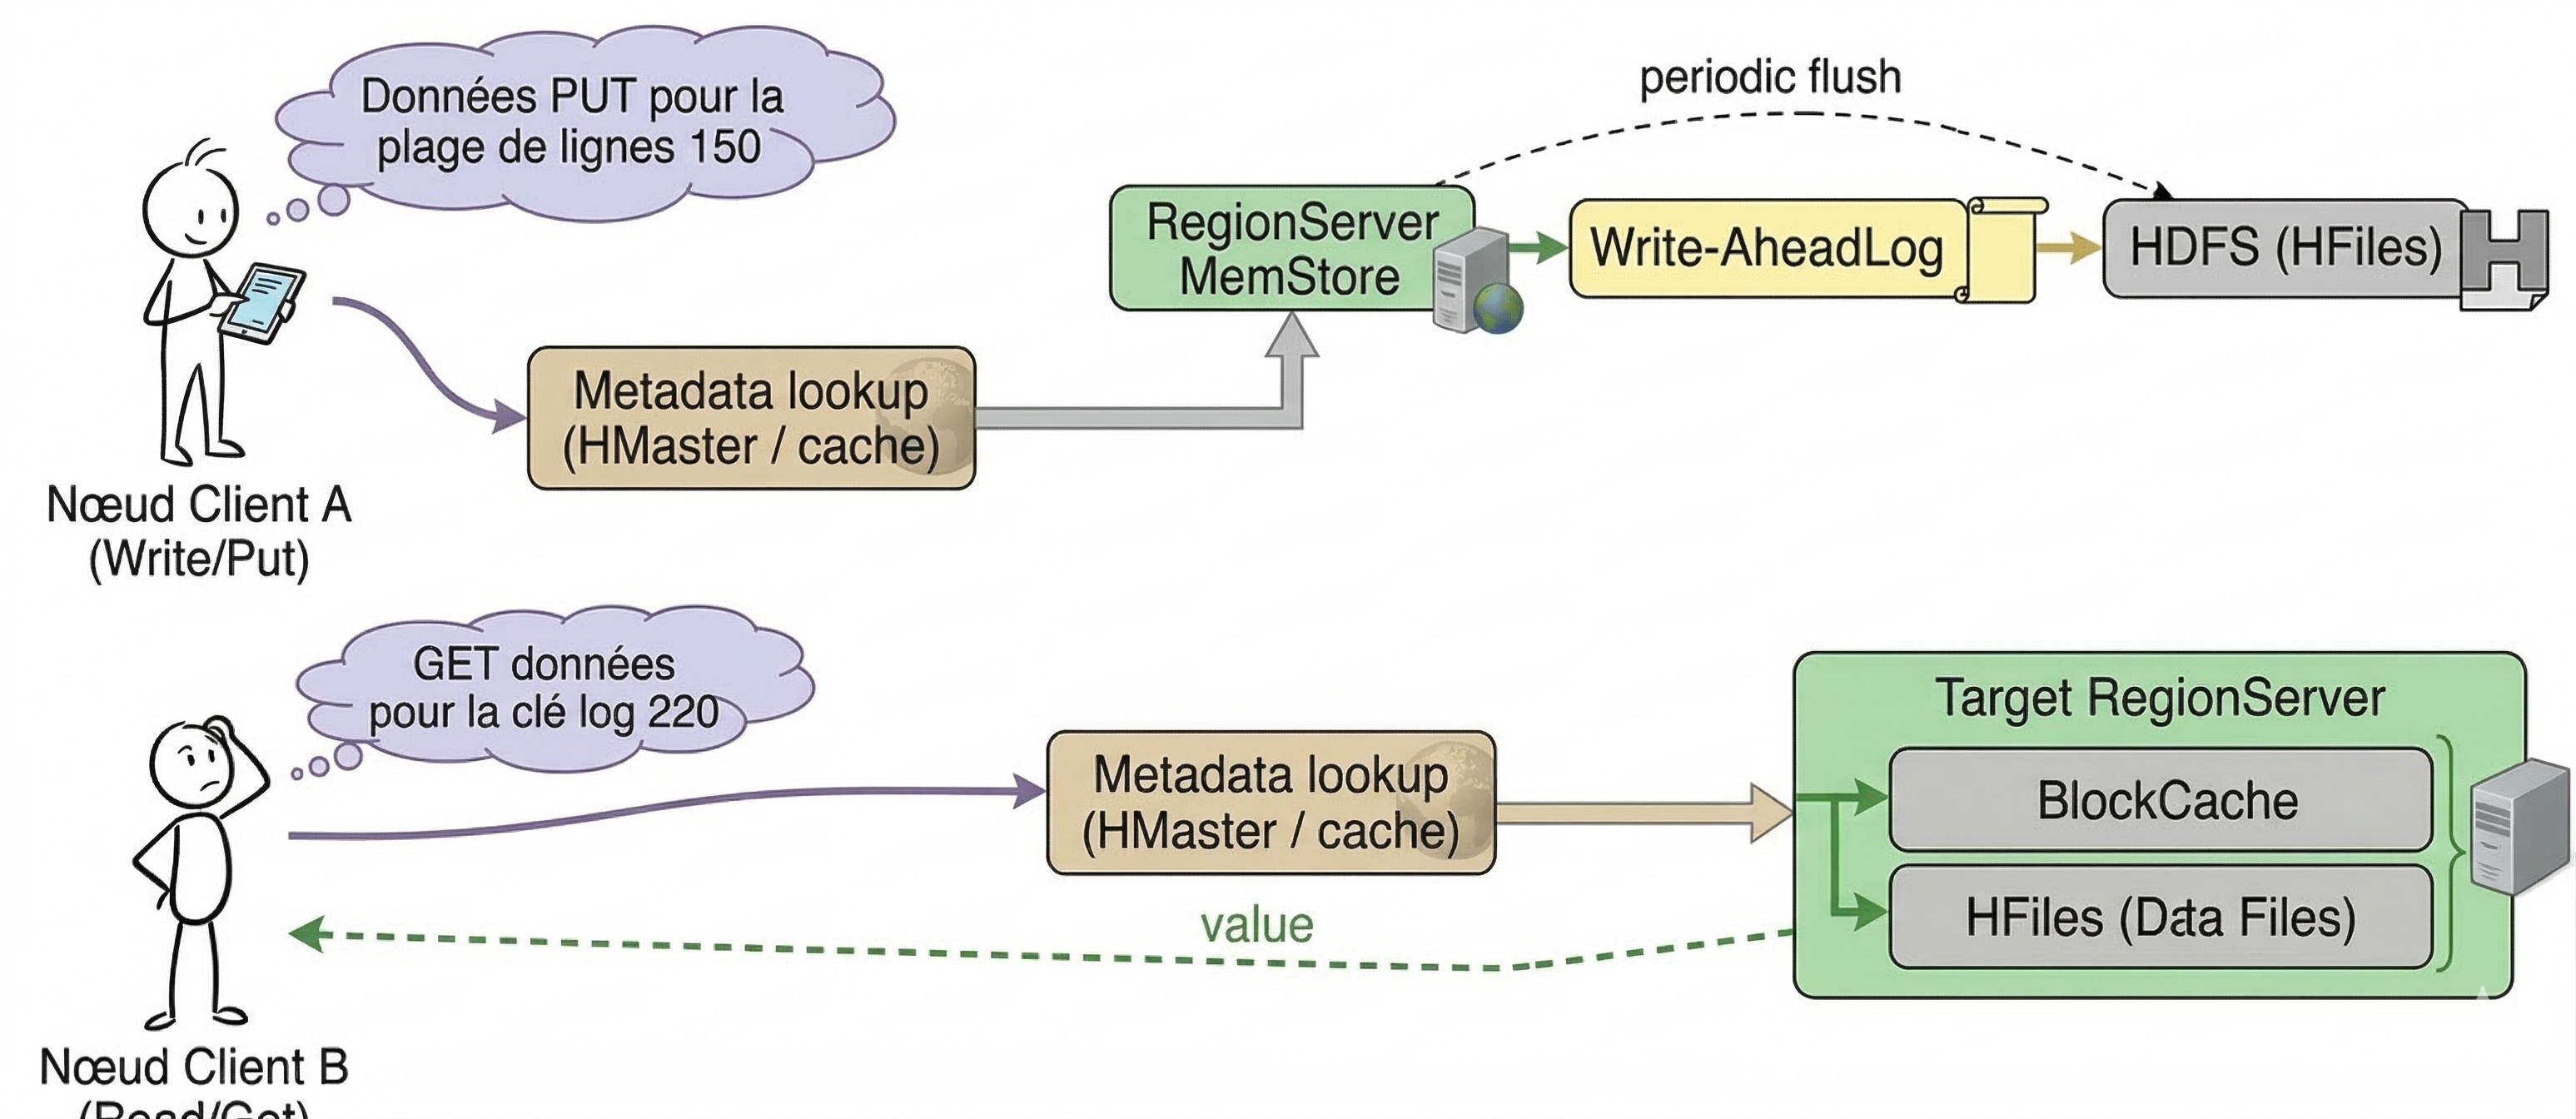
\includegraphics[width=0.95\textwidth]{images/Gemini_Generated_Image_put_get_HBase.png}
\caption{Diagramme simplifi\'e des flux \texttt{PUT}/\texttt{GET} dans HBase. Pour un \texttt{PUT} (client A), le client commence par une r\'esolution de m\'etadonn\'ees (HMaster/cache), envoie l'\'ecriture au RegionServer cibl\'e (MemStore), puis la donn\'ee est s\'ecuris\'ee via le Write-Ahead Log avant d'\^etre persist\'ee sous forme de HFiles sur HDFS (flush p\'eriodique). Pour un \texttt{GET} (client B), le client r\'esout d'abord la localisation de la r\'egion, interroge le RegionServer cible, puis la valeur est servie depuis le BlockCache ou les HFiles selon la disponibilit\'e des blocs. Cette vue fournit une lecture op\'erationnelle concise des chemins d'\'ecriture et de lecture dans HBase.}
\label{fig:hbase_put_get_simplified_flow}
\end{figure}

Cette d\'ecomposition met en \`evidence un point important pour l'analyse comparative avec les DHT : la localisation est semi-indirecte (m\'etadonn\'ees puis acc\`es direct), ce qui r\'eduit le co\^ut de routage apr\`es initialisation, mais introduit une d\'ependance \`a la qualit\'e de la gestion des r\'egions et du cache client.

Le \emph{HBase Master} g\`ere le cluster (allocation des r\'egions, \'equilibrage, d\'etection de pannes), tandis que les \emph{RegionServers} stockent les donn\'ees et ex\'ecutent les lectures/\'ecritures. Cette s\'eparation simplifie l'administration et le contr\^ole op\'erationnel.

\subsubsection*{Mod\`ele de donn\'ees et espace d'adressage}

Le mod\`ele est orient\'e colonnes (tables, \emph{rows}, familles de colonnes). Les \emph{row keys} ordonn\'ees lexicographiquement d\'efinissent l'espace d'adressage : excellent pour les scans et les requ\^etes par plages, mais sensible au design des cl\'es.


\subsubsection{M\'ecanismes internes : partitionnement et gestion des pannes}

Deux m\'ecanismes portent la scalabilit\'e et la durabilit\'e : partitionnement par r\'egions et r\'eaffectation apr\`es panne.

\subsubsection*{Partitionnement horizontal par plages de cl\'es}

Les tables sont d\'ecoup\'ees en r\'egions couvrant des plages continues de \emph{row keys}. Avec la croissance des donn\'ees, \emph{region splitting} r\'epartit la charge entre RegionServers. Limite cl\'e : des cl\'es monotones (ex.~timestamps) cr\'eent des \emph{hotspots} et du \emph{data skew} (\emph{storage skew}/\emph{access skew}).

Par rapport au \emph{consistent hashing} des DHT (distribution pseudo-al\'eatoire), HBase choisit un partitionnement d\'eterministe par ordre de cl\'es.

\subsubsection*{Gestion des pannes et r\'eaffectation}

En cas de panne d'un RegionServer, le Master (avec ZooKeeper) r\'eassigne les r\'egions. Avec le \emph{WAL} et HDFS, la reconstruction est robuste. Ce mod\`ele est centralis\'e, contrairement \`a la r\'eorganisation incr\'ementale des DHT.


\subsubsection{Avantages et limites}

\textbf{Avantages.} Coh\'erence forte par ligne, scans s\'equentiels performants et scalabilit\'e horizontale via \emph{region splitting} et ajout de RegionServers.

\textbf{Limites.} Le design des cl\'es reste critique (risques de \emph{hotspot} et de \emph{data skew}), et l'exploitation est plus lourde qu'une DHT pure (HDFS, ZooKeeper, tuning et supervision).